\documentclass{article}
\usepackage[T1]{fontenc}
\usepackage{lmodern}
\usepackage{graphicx}
\usepackage{amsmath,amssymb}
\usepackage[a4paper,margin=2cm]{geometry}
\usepackage[absolute,overlay]{textpos}
\setlength{\TPHorizModule}{1mm}
\setlength{\TPVertModule}{1mm}
\usepackage[indonesian]{babel}
\usepackage{hyperref}
\setlength{\emergencystretch}{2em}
% unit: Halaman 42

\begin{document}

% === Halaman 42 (llm) ===

\section*{InvMixColumns()}

\vspace{10mm}

\[
\begin{bmatrix}
0\text{E} & 0\text{B} & 0\text{D} & 09 \\
09 & 0\text{E} & 0\text{B} & 0\text{D} \\
0\text{D} & 09 & 0\text{E} & 0\text{B} \\
0\text{B} & 0\text{D} & 09 & 0\text{E}
\end{bmatrix}
\begin{bmatrix}
s_{0,0} & s_{0,1} & s_{0,2} & s_{0,3} \\
s_{1,0} & s_{1,1} & s_{1,2} & s_{1,3} \\
s_{2,0} & s_{2,1} & s_{2,2} & s_{2,3} \\
s_{3,0} & s_{3,1} & s_{3,2} & s_{3,3}
\end{bmatrix} = 
\begin{bmatrix}
s'_{0,0} & s'_{0,1} & s'_{0,2} & s'_{0,3} \\
s'_{1,0} & s'_{1,1} & s'_{1,2} & s'_{1,3} \\
s'_{2,0} & s'_{2,1} & s'_{2,2} & s'_{2,3} \\
s'_{3,0} & s'_{3,1} & s'_{3,2} & s'_{3,3}
\end{bmatrix}
\]

% deskripsi: Persamaan matriks untuk operasi InvMixColumns dalam algoritma AES, menunjukkan perkalian matriks konstanta dengan matriks state s untuk menghasilkan state baru s'.
% bbox normalisasi: [0.1020, 0.3600, 0.8870, 0.6420]
\begin{textblock*}{164.85mm}(21.42mm,106.92mm)
\noindent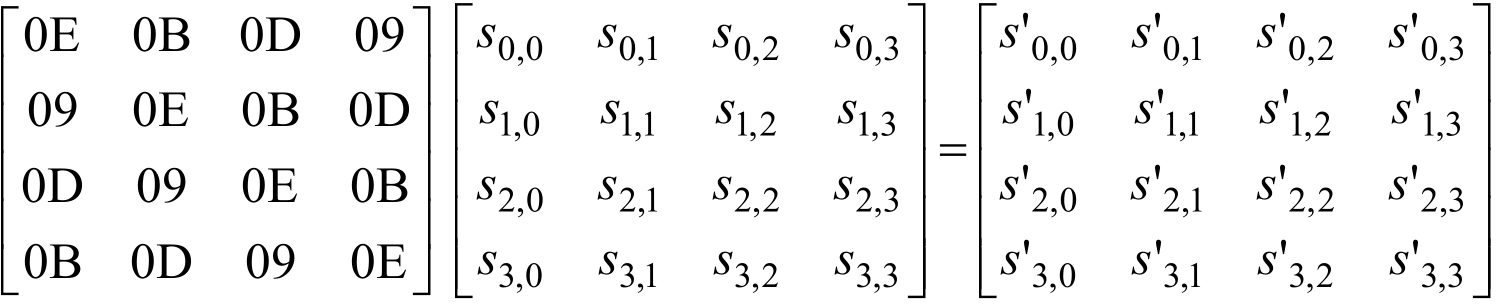
\includegraphics[width=164.85mm,height=83.75mm]{../../images/llm/page_042_img_01.png}%
\end{textblock*}

\end{document}
